%%%%%%%%%%%%%%%%%%%%%%%%%%%%%%%%%%%%%%%%%%%%%%%%%%%%%%%%%%%%%%%%%%%%%%%%%%%%
%% Trim Size: 9.75in x 6.5in
%% Text Area: 8in (include Runningheads) x 5in
%% ws-mpla.tex   :   29-9-2008
%% TeX file to use with ws-mpla.cls written in Latex2E.
%% The content, structure, format and layout of this style file is the
%% property of World Scientific Publishing Co. Pte. Ltd.
%% Copyright 1995, 2002 by World Scientific Publishing Co.
%% All rights are reserved.
%%%%%%%%%%%%%%%%%%%%%%%%%%%%%%%%%%%%%%%%%%%%%%%%%%%%%%%%%%%%%%%%%%%%%%%%%%%%
%%

\documentclass{ws-mpla}
\usepackage{cite}
%\usepackage[super]{cite}
\usepackage{graphicx}
\usepackage{color,url}
\begin{document}

\markboth{Jongwon Lim, Chih-Ting Lu, Jae-hyeon Park, and Jiwon Park}{IMPLEMENTATION OF THE ATLAS-SUSY-2018-04 ANALYSIS IN THE MADANALYSIS 5 FRAMEWORK}

%%%%%%%%%%%%%%%%%%%%% Publisher's Area please ignore %%%%%%%%%%%%%%
\catchline{}{}{}{}{}
%%%%%%%%%%%%%%%%%%%%%%%%%%%%%%%%%%%%%%%%%%%%%%%%%%%%%%%%%%%%%%%%%%%

\title{IMPLEMENTATION OF THE ATLAS-SUSY-2018-04 ANALYSIS IN THE MADANALYSIS 5 FRAMEWORK}

\author{\footnotesize Jongwon Lim}
\address{
  Department of Physics, Hanyang University, Seoul 04763, Republic of Korea}

\author{\footnotesize Chih-Ting Lu}
\address{
  School of Physics, KIAS, Seoul 02455, Republic of Korea}

\author{\footnotesize Jae-hyeon Park}
\address{
  School of Physics, KIAS, Seoul 02455, Republic of Korea}

\author{\footnotesize Jiwon Park}
\address{
  Department of Physics, Hanyang University, Seoul 04763, Republic of Korea}
\maketitle

\pub{Received (Day Month Year)}{Revised (Day Month Year)}

\begin{abstract}
We present the MADANALYSIS 5 implementation and validation of the ATLAS-SUSY-2018-04 search.
This ATLAS analysis targets the search for direct stau production in events with two hadronic tau leptons and {\color{blue}uses a dataset of LHC proton-proton collisions with an integrated luninosity of 139 fb$^{-1}$} at a center-of-mass energy of 13 TeV.
The validation of our reimplementation relies on a comparison of our cutflow predictions with the official ATLAS results in the context of two supersymmetry-inspired simplified {\color{blue}model benchmarks} in which the Standard Model is extended by a neutralino and a stau decaying into a tau lepton and a neutralino.
\keywords{supersymmetry; stau; hadronic tau lepton.}
\end{abstract}

%\ccode{PACS Nos.: include PACS Nos.}

\section{Introduction}

\begin{figure}[t]
  \centerline{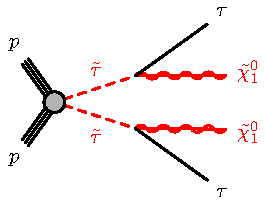
\includegraphics[width=2.0in]{fig_01}}
  \vspace*{8pt}
  \caption{The Feynman diagram for the process $pp\rightarrow\tilde{\tau}\tilde{\tau}\rightarrow\tilde{\chi}^0_1\tilde{\chi}^0_1\tau\tau$.\protect\label{fig:fig_01}}
\end{figure}

In this note, we describe the validation of the implementation, in MADANALYSIS 5 framework~\cite{Conte:2018vmg,Dumont:2014tja,Conte:2014zja,Conte:2012fm}, of the ATLAS-SUSY-2018-04 search~\cite{Aad:2019byo} for direct stau production in two hadronic $\tau +E^{miss}_T$ events. 
This process is illustrated by the representative Feynman diagram of Fig.~\ref{fig:fig_01}. 
This analysis is based on a data sample of LHC proton-proton collisions at a center-of-mass energy of 13 TeV corresponding to an integrated luminosity of $139 fb^{-1}$.

For the validation of our reimplementation, we have focused on the sector of sparticles with only electroweak interactions. 
The lightest neutralino ($\tilde{\chi}^0_1$) is taken as the lightest supersymmetric particle (LSP). 
The stau-left ($\tilde{\tau}_L$) and stau-right ($\tilde{\tau}_R$) are assumed to be mass degenerate without mixing.  Therefore the gauge eigenstates ($\tilde{\tau}_L$,$\tilde{\tau}_R$) coincide with the mass eigenstates ($\tilde{\tau}_1$,$\tilde{\tau}_2$). 
Furthermore, in order to suppress other decay modes of stau, the masses of all charginos and neutralinos are set to 2.5 TeV except for the $\tilde{\chi}^0_1$. 
Hence, the single kinematically allowed decay mode of stau is 
\begin{equation}
\tilde{\tau}\rightarrow\tilde{\chi}^0_1 \tau 
\end{equation}
 

\section{Description of the analysis}

This analysis targets a final state containing two hadronic tau leptons with a certain amount of missing transverse energy. 
The kinematics of {\color{blue}hadronic} di-$\tau +E^{miss}_T$ system is used to reduce the contributions from Standard Model backgrounds. 
First, all the objects are reconstructed and defined. Then a sequence of event selections for the signal final state is applied.

\subsection{Object definitions}

Jets are reconstructed by means of the anti-$k_t$ algorithm~\cite{Cacciari:2008gp} with a radius parameter set to $R=0.4$. This analysis focuses on jets whose transverse momentum $p^j_T$ and pseudorapidity $\eta^j$ fullfill
\begin{equation}
p^j_T > 20\textrm{ GeV}\quad \textrm{and}\quad |\eta^j| < 2.8.
\end{equation} 
Moreover, {\color{blue}the selected jets which are required to satisfy 
\begin{equation}
p^b_T > 20 \textrm{ GeV}\quad \textrm{and}\quad |\eta^b| < 2.5,
\end{equation}
are tagged as originating from the fragmentation of $b$-quarks.}
A working point with the average $b$-tagging efficiency of $77\%$ is used. This working point corresponds to a $c$-jet and light-jet rejection of $4.9$ and $110$, respectively.

Electron candidates are required to have a transverse momentum $p^e_T$ and pseudorapidity $\eta^e$ obeying
\begin{equation}
p^e_T > 17 \textrm{ GeV}\quad \textrm{and}\quad |\eta^e| < 2.47.
\end{equation}
Furthermore, all electron candidates are required to have both track and calorimeter isolations
to reduce the number of jets misidentified as charged leptons.
For the track isolation, the scalar sum of the $p_T$ of tracks inside a variable-size cone around the electron (excluding its own track) is required to satisfy
\begin{equation}
\sum p_{T,\textrm{tracks}}/p^e_T < 0.15 ,
\end{equation}
with the cone size
\begin{equation}
\Delta R=\min(10\textrm{ GeV}/p^e_T,0.2) .
\end{equation}
For the calorimeter isolation,
the sum of the transverse energy of the calorimeter energy clusters is required to satisfy
\begin{equation}
\sum E_{T,\textrm{calorimeter}}/p^e_T < 0.2 ,
\end{equation}
in a cone of size
\begin{equation}
\Delta R=0.2
\end{equation}
around the electron, excluding the energy from the electron itself.
For electrons with a high transverse momentum
$ p^e_T > 200\textrm{ GeV} $,
only an upper limit instead is imposed on the transverse energy of the calorimeter energy clusters so that
\begin{equation}
\sum E_{T,\textrm{tracks}} < \max(0.015\times p^e_T,3.5\textrm{ GeV}) ,
\end{equation}
in a cone of
\begin{equation}
\Delta R=0.2
\end{equation}
around the electron.

Muon candidate definition is similar to that for electrons, although with slightly looser thresholds,
$p^{\mu}_T > 14 \textrm{ GeV}$ and $|\eta^{\mu}| < 2.7$.
The condition of the track isolation is the same, i.e.\
$\sum p_{T,\textrm{tracks}}/p^{\mu}_T < 0.15$,
with an altered cone size
$\Delta R=\min(10\textrm{ GeV}/p^{\mu}_T,0.3)$.
The condition of the calorimeter isolation is changed to
$\sum E_{T,\textrm{tracks}}/p^{\mu}_T < 0.3$
with the same cone size $\Delta R=0.2$.

Tau lepton candidates are reconstructed with one or three associated charged pion tracks (prongs). %$\sum_i e_i (\textrm{tracks}) = \pm 1$.
%For 1-prong (3-prong) $\tau$ lepton candidates, the signal efficiencies are $75\%$($60\%$) and $60\%$($45\%$) for the \textit{medium} and \textit{tight} working points, respectively.
For 1-prong (3-prong) $\tau$ lepton candidates, the signal efficiencies are $75\%$ and $60\%$ for the \textit{medium} working points. 
{\color{blue}The \textit{tight} working point efficiencies are directly taken from the official ATLAS cutflow table in this recasting.}
%Due to the technical restriction, the \textit{tight} working point efficiencies are directly taken from the official ATLAS cutflow table. %Should add more details
The baseline tau lepton candidates are required to have 
\begin{equation}
p^{\tau}_T > 50(40) \textrm{ GeV}\quad \textrm{and}\quad |\eta^{\tau}| < 2.5
\end{equation}
for the leading (subleading) ones and the transition region between the barrel and endcap calorimeters ($ 1.37 < |\eta^{\tau}| < 1.52 $) is excluded.

Finally, some overlap removal conditions are in order which are consistent with the analysis code provided in HEPData\cite{hepdata}. Electrons are removed if they overlap so closely with another electron that $\Delta R(e,e) < 0.05$. Tau candidates are discarded if they overlap with a light lepton, i.e.\ $\Delta R(\tau,e/\mu) < 0.2$. If an electron overlaps with a muon such that $\Delta R(e,\mu) < 0.01$, the muon is retained. If a jet is found to overlap with a light lepton leading to $\Delta R(j,e/\mu) < 0.2$, the jet is discarded. For overlapping light leptons and jets with $\Delta R(e/\mu,j) < 0.4$, the jet is kept. Lastly, jets are removed if they overlap with a tau such that $\Delta R(j,\tau) < 0.4$.


\subsection{Event selection}
%The analysis contains two \textit{medium} tau lepton candidates with opposite-sign electric charge (OS). All events are required to pass either an \textit{asymmetric di-$\tau$} trigger for the low stau mass region (SR-lowMass) or a combined \textit{di-$\tau +E^{miss}_T$} ($E^{miss}_T > 150$ GeV) trigger for the high stau mass region (SR-highMass). The trigger efficiencies about $80\%$ are applied in our recasting with the following offline $p_T$ thresholds for the leading (subleading) tau lepton candidates in Table~\ref{tab:trig-eff}.
%Events with the third \textit{medium} tau lepton or any light lepton are rejected. 
%On the other hand, values of $75 < E^{miss}_T < 150$ GeV are required for SR-lowMass to increase signal sensitivity.

%Furthermore, $b$-jet veto is applied to reject events from top quark associated processes. The reconstructed invariant mass of the two leading tau lepton candidates, $m(\tau_1,\tau_2)$, larger than $120$ GeV is required for removing tau lepton pair from low-mass resonances, $Z$ boson, and Higgs boson events ($Z/H$ veto).

%Here mostly re-arranged sentences from above paragraphs
The events with exactly two \textit{medium} tau lepton candidates with opposite-sign (OS) electric charge are selected.
Then, $b$-jet veto is applied to reject events from top quark associated processes.
Also, the events with additional light lepton (muon or electron) are rejected.
The reconstructed invariant mass of the two leading {\color{blue}hadronic taus}, $m(\tau_1,\tau_2)$, larger than $120$ GeV is required for removing tau lepton pair from low-mass {\color{blue}$Z/H$ resonances}.

All events are required to pass either an \textit{asymmetric di-$\tau$} trigger for the low stau mass region or a combined \textit{di-$\tau +E^{miss}_T$} ($E^{miss}_T > 150$ GeV) trigger for the high stau mass region (Trigger and offline cuts).
The trigger efficiencies about $80\%$ are applied in our recasting with the following offline $p_T$ thresholds for the leading (subleading) tau lepton candidates in Table~\ref{tab:trig-eff}.

\begin{table}[h!]
  \tbl{Offline $p_T$ thresholds for the leading (subleading) tau lepton candidates of \textit{asymmetric di-$\tau$} and \textit{di-$\tau +E^{miss}_T$} triggers with efficiencies about $80\%$.}
  {\begin{tabular}{@{}c c c@{}} \toprule
  Year & \textit{asymmetric di-$\tau$} & \textit{di-$\tau +E^{miss}_T$} \\
  \colrule
 2015-2017 & $95(60)$ GeV & $50(40)$ GeV \\
 2018 & $95(75)$ GeV & $75(40)$ GeV \\ 
  \botrule
  \end{tabular}\label{tab:trig-eff} }
\end{table}

In {\color{blue}low mass} region, values of $75 < E^{miss}_T < 150$ GeV are required to increase signal sensitivity.
Also, two selected tau leptons are required to be tight tagged.
The selection efficiency of two taus passing the \textit{tight} working point on top of two {\color{blue}tagged tau leptons with the \textit{medium} working point is} taken from official ATLAS cutflow table as a ratio of raw number of event before and after applying cut. {\color{blue}The  tau tagging efficiency of \textit{tight} working point} is then applied as a probability per tau lepton by a square root of the efficiency.
On the other hand, in {\color{blue}high mass} region, the tight tagging efficiency is applied in the same manner as {\color{blue}low mass} region, but allowing at least one of two tau leptons passing the tight selection.

The \textit{stransverse mass} $m_{T2}$ variable is defined as
%\footnote{
%Notice $m_{T2}$ calculation is done with MADANALYSIS 5 function ($PHYSICS\rightarrow Transverse\rightarrow MT2(vec1,vec2,E^{miss}_T,m_{invisible})$)
%}
\begin{equation}
m_{T2} =min_{\mathbf{q}_T}
\left[
max(m_{T,\tau_1}(\mathbf{p}_{T,\tau_1},\mathbf{q}_T),m_{T,\tau_2}(\mathbf{p}_{T,\tau_2},\mathbf{p}^{miss}_T -\mathbf{q}_T))
\right],
\end{equation}   
where $\mathbf{p}_{T,\tau_1}$ and $\mathbf{p}_{T,\tau_2}$ are the transverse momenta of the two tau lepton candidates, and the transverse momentum vector of one of the invisible particle, $\mathbf{q}_T$, is chosen to minimize the larger of the two transverse mass $m_{T,\tau_1}$ and $m_{T,\tau_2}$. The transverse mass $m_T$ is defined by
\begin{equation}
m_{T}(\mathbf{p}_T,\mathbf{q}_T) = \sqrt{2(p_T q_T -\mathbf{p}_T\cdot\mathbf{q}_T)}.
\end{equation} 
A lower bound on the $m_{T2}$ will be imposed to reduce contributions from $t\overline{t}$ and $WW$ events.
Finally, the two tau lepton candidates are required to satisfy $\Delta R(\tau_1,\tau_2) < 3.2$, $|\Delta\phi (\tau_1,\tau_2)| > 0.8$ and $m_{T2} > 70$ GeV to further suppress contributions from SM backgrounds.


%\begin{table}[t]
%  \tbl{Please use this template for tables.}
%  {\begin{tabular}{@{}cccc@{}} \toprule
%  Piston mass & Analytical frequency & TRIA6-$S_1$ model &
%  \% Error \\
%  & (Rad/s) & (Rad/s) \\
%  \colrule
%  1.0\hphantom{00} & \hphantom{0}281.0 & \hphantom{0}280.81 & 0.07 \\
%  0.1\hphantom{00} & \hphantom{0}876.0 & \hphantom{0}875.74 & 0.03 \\
%  0.01\hphantom{0} & 2441.0 & 2441.0\hphantom{0} & 0.0\hphantom{0} \\
%  0.001 & 4130.0 & 4129.3\hphantom{0} & 0.16\\ \botrule
%  \end{tabular}\label{ta1} }
%\end{table}


\section{Validation}

\subsection{Event generation}

In order to validate our analysis, we rely on the MSSM UFO model file~\cite{Duhr:2011se} from Feynrules model database~\cite{Alloul:2013bka}. 
Two benchmark points with masses $ m(\tilde{\tau},\tilde{\chi}^0_1)=(120,1) $ GeV and $ (280,1) $ GeV are used in this note to illustrate the validation of our reimplementation. 
We make use of MADGRAPH5 aMC@NLO version 2.6.7~\cite{Alwall:2014hca} for hard-scattering event generation in which leading-order matrix elements are convoluted with the {\color{blue}LO set of} NNPDF2.3~\cite{Ball:2012cx} parton distribution function (PDF) set. The signal includes the emission of up to two additional partons. We apply the MLM scheme~\cite{Mangano:2006rw,Alwall:2008qv} of the ME-PS matching with $xqcut = m_{\tilde{\tau}}/4$.
The PYTHIA8 version 8.244~\cite{Sjostrand:2007gs} with $A14$ tune has been used for the simulation of the parton showering and hadronization. The simulation of the detector response has been performed by using DELPHES-3.4.2~\cite{deFavereau:2013fsa}, that relies on FASTJET~\cite{Cacciari:2011ma} for object reconstruction.
The modified delphes card has been used with an appropriate tuned detector card.
{\color{red}For example, the loosened isolation criteria are applied to cover all offline object definitions.(I don't understand Jack's comment here)}
\textcolor{magenta}{It might be unclear what you mean by ``the loosened isolation criteria''.  I do not find its definition in the text either.}
%And the radius parameter of jet and minimum transverse momentum are lowered to 0.4 and 15 GeV with updating $b$ and tau tagging efficiencies.
%Also, UniqueObjectFinder is disabled for overlap removal which is done in MADANALYSIS5.
Finally, we have used the {\color{blue}MADANALYSIS 5 framework for recasting} the signal selection efficiencies.



\subsection{Comparison with the official results}
In Table~\ref{tab:120GeV} and~\ref{tab:280GeV}, we compare the results obtained with our implememtation to the official raw event numbers in the auxiliary tables provided by the ATLAS collaboration for the benchmark points with masses $m(\tilde{\tau},\tilde{\chi}^0_1)=(120,1) $ and $(280,1)$ GeV, respectively. 
For each cut, we have calculated the related efficiency defined as 
\begin{equation}
\epsilon_i =\frac{n_i}{n_{i-1}}
\end{equation}
where $ n_i $ and $ n_{i-1} $ {\color{blue}refer to} the event number after and before the considered cut, respectively.
%
On the other hand, we have also calculated the differences between $ \epsilon_i (MA5)$ and $ \epsilon_i (ATLAS)$ with the definition as
\begin{equation}
diff. = \frac{\epsilon_i (MA5)-\epsilon_i (ATLAS)}{\epsilon_i (ATLAS)}
\end{equation}


\begin{table}[h!]
  \tbl{Validation checks of the cut flows for $ \tilde{\tau}\tilde{\tau} $ production with $ m(\tilde{\tau},\tilde{\chi}^0_1) = (120,1) $ GeV.}
  {\begin{tabular}{@{}c c c c c c@{}} \toprule
\hline
\multicolumn{6}{c}{ \textbf{$ \tilde{\tau}\tilde{\tau} $ production with $ m(\tilde{\tau},\tilde{\chi}^0_1) = (120,1) $ GeV} }\\
\hline\hline
 & ATLAS($N_{raw}$) & $\epsilon_i$($\%$) & MA5($N_{raw}$) & $\epsilon_i$($\%$) & diff.($\%$) \\
\hline\hline

2 medium $\tau$ (OS) and 3rd baseline $\tau$ veto & 22493 & & 26016 & & \\ \hline
$b$-jet veto & 22148 & 98.47 & 25429 & 97.74 & $-0.74$ \\ \hline
Light lepton veto & 22109 & 99.82 & 25414 & 99.94 & 0.12 \\ \hline
$Z/H$-veto & 18188 & 82.27 & 21082 & 82.95 & 0.83 \\ \hline
%
\multicolumn{5}{c}{ \textbf{low mass region} }\\\hline
%
Trigger and offline cuts & 6512 & 35.80 & 8144 & 38.63 & 7.91 \\ \hline
$ 75 < E^{miss}_T < 150 $ GeV & 2228 & 34.21 & 2840 & 34.87 & 1.93 \\ \hline
2 tight $\tau$ & 1565 & 70.24 & 1973 & 69.47 & $-1.10$ \\ \hline
$ |\Delta\phi(\tau,\tau)| > 0.8 $ & 1564 & 99.94 & 1965 & 99.59 & $-0.35$ \\ \hline
$ |\Delta R(\tau,\tau)| < 3.2 $ & 1429 & 91.37 & 1796 & 91.40 & 0.03 \\ \hline
$ m_{T2} > 70 $ GeV & 280 & 19.59 & 537 & 29.90 & 52.63 \\ \hline
All &  & 1.24 &  & 2.06 & 66.13 \\ \hline
%
\hline
\multicolumn{5}{c}{ \textbf{high mass region} }\\\hline
%
Trigger and offline cuts & 1272 & 6.99 & 1649 & 7.82 & 11.87 \\ \hline
$ \geq 1 $ tight $\tau$ & 1249 & 98.19 & 1590 & 96.42 & $-1.80$ \\ \hline
$ |\Delta\phi(\tau,\tau)| > 0.8 $ & 1236 & 98.96 & 1560 & 98.11 & $-0.86$ \\ \hline
$ |\Delta R(\tau,\tau)| < 3.2 $ & 1132 & 91.59 & 1408 & 90.26 & $-1.45$ \\ \hline
$ m_{T2} > 70 $ GeV & 170 & 15.02 & 326 & 23.15 & 54.13 \\ \hline
All &  & 0.76 &  & 1.25 & 64.47 \\ \botrule
\end{tabular}
\label{tab:120GeV} }
\end{table}

\begin{table}[h!]
  \tbl{Validation checks of the cut flows for $ \tilde{\tau}\tilde{\tau} $ production with $ m(\tilde{\tau},\tilde{\chi}^0_1) = (280,1) $ GeV.}
  {\begin{tabular}{@{}c c c c c c@{}} \toprule
\hline
\multicolumn{6}{c}{ \textbf{$ \tilde{\tau}\tilde{\tau} $ production with $ m(\tilde{\tau},\tilde{\chi}^0_1) = (280,1) $ GeV} }\\
\hline\hline
 & ATLAS($N_{raw}$) & $\epsilon_i$($\%$) & MA5($N_{raw}$) & $\epsilon_i$($\%$) & diff.($\%$) \\
\hline\hline

2 medium $\tau$ (OS) and 3rd baseline $\tau$ veto & 3980 & & 35261 & & \\ \hline
$b$-jet veto & 3903 & 98.07 & 34338 & 97.38 & $-0.70$ \\ \hline
Light lepton veto & 3888 & 99.62 & 34308 & 99.91 & 0.29 \\ \hline
$Z/H$-veto & 3382 & 86.99 & 30356 & 88.48 & 1.71 \\ \hline
%
\multicolumn{5}{c}{ \textbf{low mass region} }\\\hline
%
Trigger and offline cuts & 1920 & 56.77 & 17468 & 57.54 & 1.36 \\ \hline
$ 75 < E^{miss}_T < 150 $ GeV & 738 & 38.44 & 6329 & 36.23 & $-5.75$ \\ \hline
2 tight $\tau$ & 512 & 69.38 & 4074 & 64.37 & $-7.22$ \\ \hline
$ |\Delta\phi(\tau,\tau)| > 0.8 $ & 512 & 100.00 & 4050 & 99.41 & $-0.59$ \\ \hline
$ |\Delta R(\tau,\tau)| < 3.2 $ & 478 & 93.36 & 3690 & 91.11 & $-2.41$ \\ \hline
$ m_{T2} > 70 $ GeV & 278 & 58.16 & 2304 & 62.44 & 7.36 \\ \hline
All &  & 6.98 &  & 6.53 & $-6.45$ \\ \hline
%
\hline
\multicolumn{5}{c}{ \textbf{high mass region} }\\\hline
%
Trigger and offline cuts & 1096 & 32.41 & 11305 & 37.24 & 14.90 \\ \hline
$ \geq 1 $ tight $\tau$ & 1076 & 98.18 & 11110 & 98.28 & $-0.10$ \\ \hline
$ |\Delta\phi(\tau,\tau)| > 0.8 $ & 1045 & 97.12 & 10643 & 95.80 & $-1.36$ \\ \hline
$ |\Delta R(\tau,\tau)| < 3.2 $ & 973 & 93.11 & 9960 & 93.58 & 0.50 \\ \hline
$ m_{T2} > 70 $ GeV & 691 & 71.02 & 7721 & 77.52 & 9.15 \\ \hline
All &  & 17.36 &  & 21.90 & 26.15 \\ \botrule
\end{tabular}
\label{tab:280GeV} }
\end{table} 


We observe that the disagreement on a cut-by-cut basis, is $8.66\%$ and $7.55\%$ before the $m_{T2}$ cut for {\color{blue}low mass} and {\color{blue}high mass regions} in Table~\ref{tab:120GeV} for $m(\tilde{\tau},\tilde{\chi}^0_1)=(120,1) $ GeV. The major part of the disagreement comes from the Trigger and offline cuts step. By lack of more public experimental information, we have not been able to validate these two steps more precisely.
\begin{figure}[h!]
  \centerline{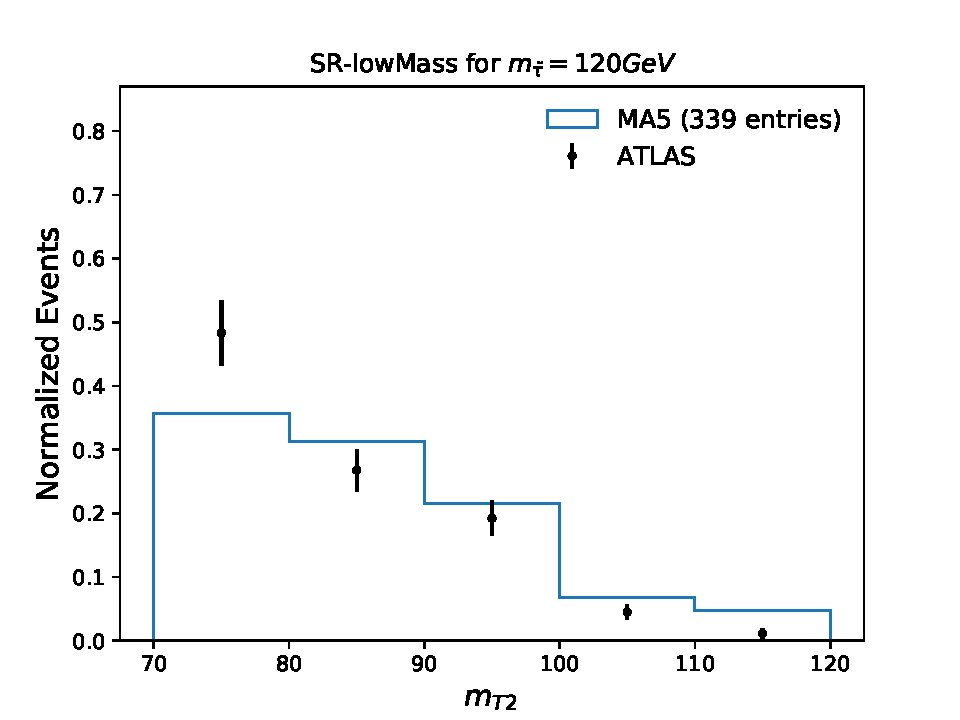
\includegraphics[width=2.0in]{m120_norm_1}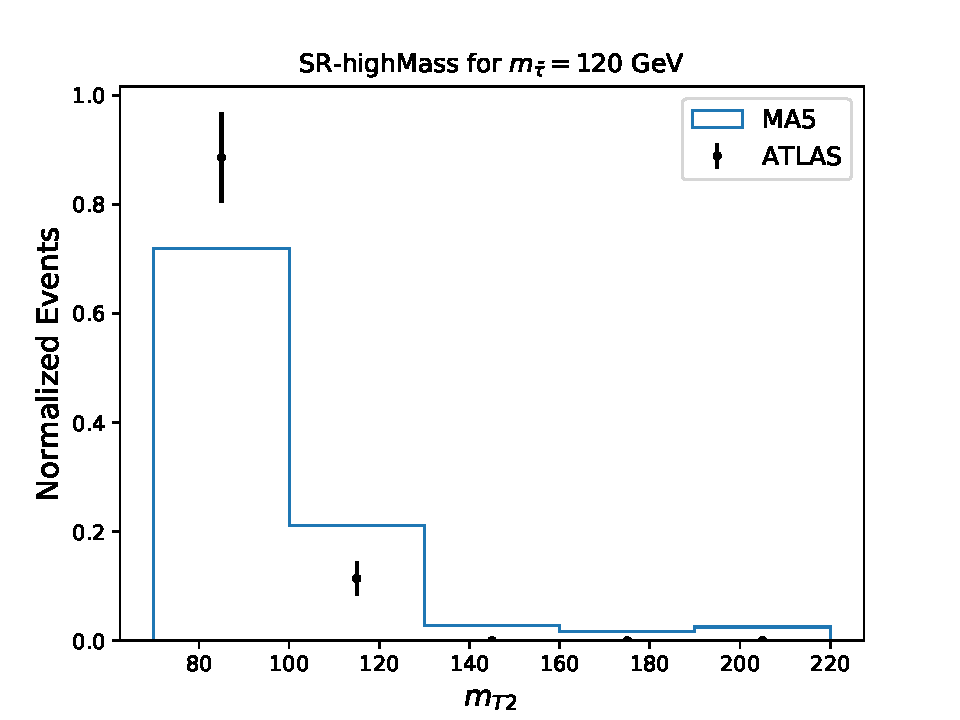
\includegraphics[width=2.0in]{m120_norm_2}}
  \vspace*{8pt}
  \caption{The $m_{T2}$ distributions for $m(\tilde{\tau},\tilde{\chi}^0_1)=(120,1)$ GeV.\protect\label{fig:m120_norm}}
\end{figure}

\begin{figure}[t]
  \centerline{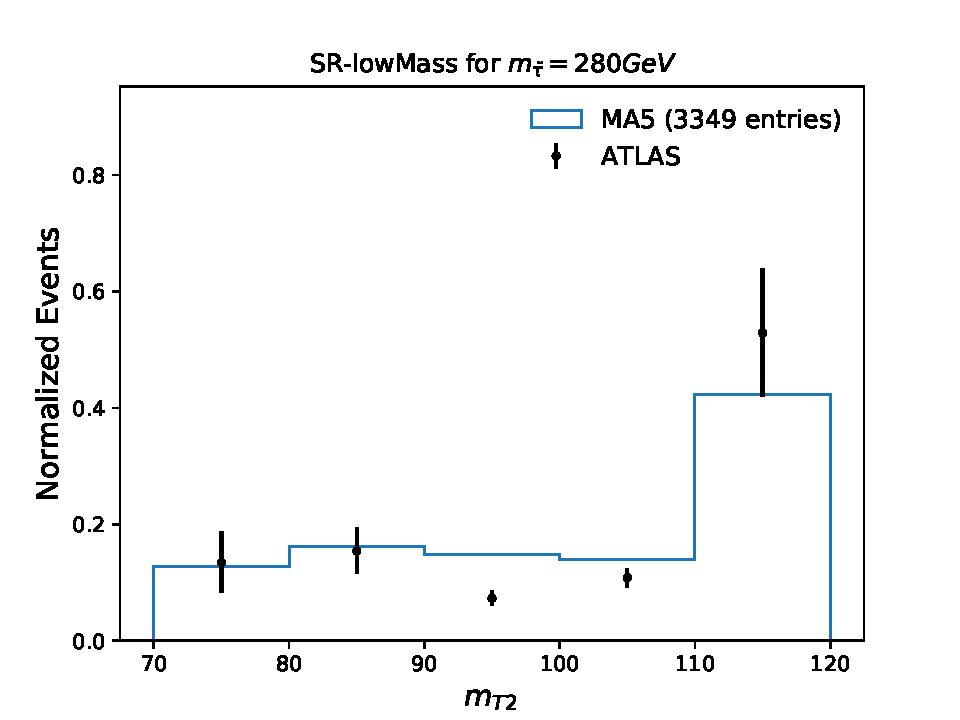
\includegraphics[width=2.0in]{m280_norm_1}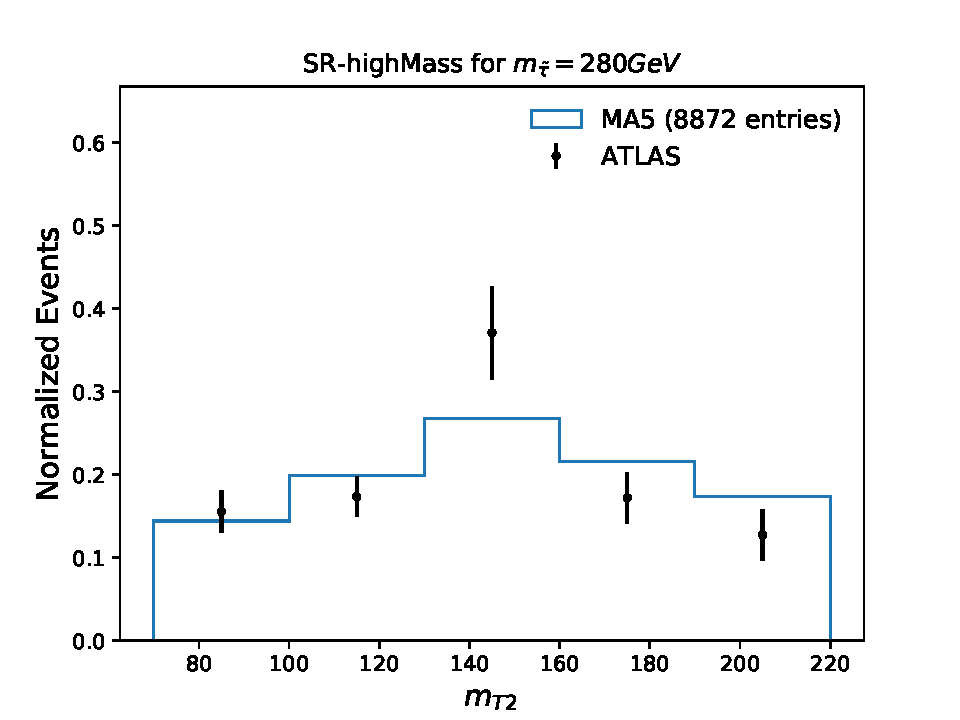
\includegraphics[width=2.0in]{m280_norm_2}}
  \vspace*{8pt}
  \caption{The $m_{T2}$ distributions for $m(\tilde{\tau},\tilde{\chi}^0_1)=(280,1)$ GeV.\protect\label{fig:m280_norm}}
\end{figure}
In Fig.~\ref{fig:m120_norm}, we {\color{blue}observed} the $m_{T2}$ distributions from ATLAS analysis are softer than our results. This causes the $m_{T2} > 70$ GeV cut looser in our reimplementation than the original ATLAS results which is taken from HEPData\cite{hepdata}.
Similarly, the disagreement on a cut-by-cut basis is $-6.45\%$ and $26.15\%$ with all cuts 
for low mass and high mass regions in Table~\ref{tab:280GeV} for $m(\tilde{\tau},\tilde{\chi}^0_1)=(280,1)$ GeV. The major parts of the disagreement come from Trigger and offline cuts, tight $\tau$ selection, and $m_{T2}$ cut steps. 
The $m_{T2}$ distributions are shown in Fig.~\ref{fig:m280_norm} for the comparison of our results with ATLAS analysis. 

%\begin{figure}[t]
%  \centerline{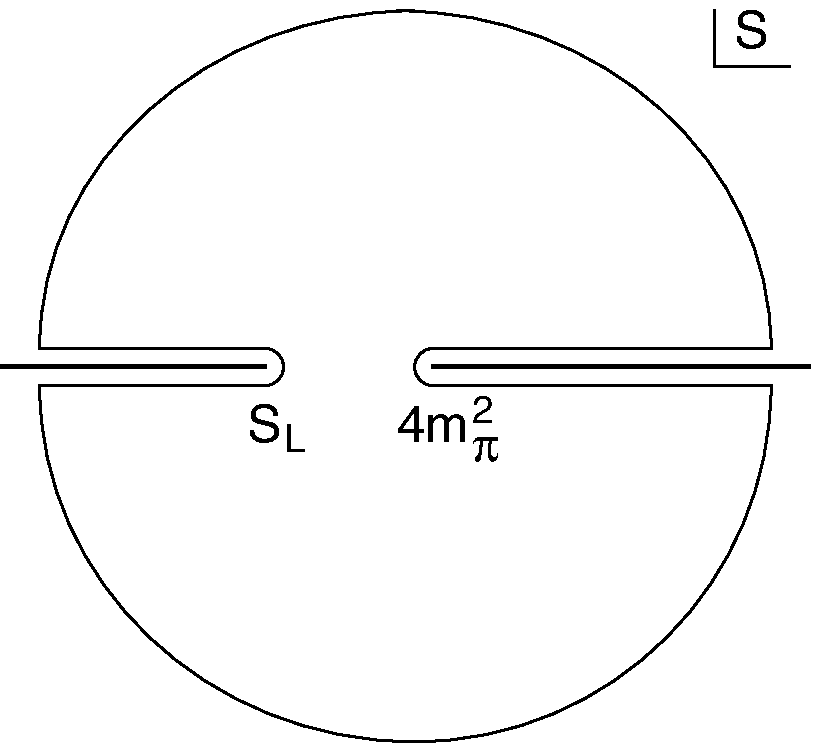
\includegraphics[width=2.0in]{mplaf1}}
%  \vspace*{8pt}
%  \caption{Please use this template for figures.\protect\label{fig1}}
%\end{figure}

\section{Conclusions}

We have implemented the ATLAS-SUSY-2018-04 search in the MADANALYSIS 5 framework. Our analysis has been validated in the context of a supersymmetry-inspired simplified benchmark model in which the Standard Model is extended by a neutralino and a stau decaying into a tau lepton and the neutralino, employing two different benchmark points in the parameter space.
By comparing our predictions for the cutflow with the official one provided by ATLAS in Ref.\cite{Aad:2019byo}, we have found an agreement for each step in Table~\ref{tab:120GeV} and~\ref{tab:280GeV} except for the ones from Trigger and offline cuts, tight $\tau$ selection, and $m_{T2}$ cut. Due to the lack of more information, we have not been able to validate these steps more precisely. 


\section*{Acknowledgments}
Dedications and funding information may be included here.
% add acknowledgments of basic kias grant (CT) and NRF grant (JP)

\begin{thebibliography}{99}
\bibitem{Conte:2018vmg}
  E.~Conte and B.~Fuks,
  Int.\ J.\ Mod.\ Phys.\ A {\bf 33} (2018) no.28,  1830027
  [arXiv:1808.00480 [hep-ph]].

\bibitem{Dumont:2014tja}
  B.~Dumont {\it et al.},
  Eur.\ Phys.\ J.\ C {\bf 75} (2015) no.2,  56
  [arXiv:1407.3278 [hep-ph]].

\bibitem{Conte:2014zja}
  E.~Conte, B.~Dumont, B.~Fuks and C.~Wymant,
  Eur.\ Phys.\ J.\ C {\bf 74} (2014) no.10,  3103
  [arXiv:1405.3982 [hep-ph]].

\bibitem{Conte:2012fm}
  E.~Conte, B.~Fuks and G.~Serret,
  Comput.\ Phys.\ Commun.\  {\bf 184} (2013) 222
  [arXiv:1206.1599 [hep-ph]].

%\cite{Aad:2019byo}
\bibitem{Aad:2019byo} 
  G.~Aad {\it et al.} [ATLAS Collaboration],
  %``Search for direct stau production in events with two hadronic $\tau$-leptons in $\sqrt{s} = 13$ TeV $pp$ collisions with the ATLAS detector,''
  Phys.\ Rev.\ D {\bf 101}, no. 3, 032009 (2020)
  doi:10.1103/PhysRevD.101.032009
  [arXiv:1911.06660 [hep-ex]].
  %%CITATION = doi:10.1103/PhysRevD.101.032009;%%
  %7 citations counted in INSPIRE as of 27 Mar 2020

%\cite{Aad:2019byo}
\bibitem{hepdata}
G.~Aad \textit{et al.} [ATLAS],
%``Search for direct stau production in events with two hadronic $\tau$-leptons in $\sqrt{s} = 13$ TeV $pp$ collisions with the ATLAS detector,''
doi:10.17182/hepdata.92006
%https://doi.org/10.17182/hepdata.92006

%\cite{Cacciari:2008gp}
\bibitem{Cacciari:2008gp} 
  M.~Cacciari, G.~P.~Salam and G.~Soyez,
  %``The anti-$k_t$ jet clustering algorithm,''
  JHEP {\bf 0804}, 063 (2008)
  doi:10.1088/1126-6708/2008/04/063
  [arXiv:0802.1189 [hep-ph]].
  %%CITATION = doi:10.1088/1126-6708/2008/04/063;%%
  %6790 citations counted in INSPIRE as of 27 Mar 2020

%\cite{Duhr:2011se}
\bibitem{Duhr:2011se} 
  C.~Duhr and B.~Fuks,
  %``A superspace module for the FeynRules package,''
  Comput.\ Phys.\ Commun.\  {\bf 182}, 2404 (2011)
  doi:10.1016/j.cpc.2011.06.009
  [arXiv:1102.4191 [hep-ph]].
  %%CITATION = doi:10.1016/j.cpc.2011.06.009;%%
  %69 citations counted in INSPIRE as of 27 Mar 2020
  
%\cite{Alloul:2013bka}
\bibitem{Alloul:2013bka} 
  A.~Alloul, N.~D.~Christensen, C.~Degrande, C.~Duhr and B.~Fuks,
  %``FeynRules  2.0 - A complete toolbox for tree-level phenomenology,''
  Comput.\ Phys.\ Commun.\  {\bf 185}, 2250 (2014)
  doi:10.1016/j.cpc.2014.04.012
  [arXiv:1310.1921 [hep-ph]].
  %%CITATION = doi:10.1016/j.cpc.2014.04.012;%%
  %1327 citations counted in INSPIRE as of 27 Mar 2020

%\cite{Alwall:2014hca}
\bibitem{Alwall:2014hca} 
  J.~Alwall {\it et al.},
  %``The automated computation of tree-level and next-to-leading order differential cross sections, and their matching to parton shower simulations,''
  JHEP {\bf 1407}, 079 (2014)
  doi:10.1007/JHEP07(2014)079
  [arXiv:1405.0301 [hep-ph]].
  %%CITATION = doi:10.1007/JHEP07(2014)079;%%
  %4502 citations counted in INSPIRE as of 27 Mar 2020

% see http://nnpdf.mi.infn.it/for-users/unpolarized-pdf-sets
%\cite{Ball:2012cx}
\bibitem{Ball:2012cx}
R.~D.~Ball, V.~Bertone, S.~Carrazza, C.~S.~Deans, L.~Del Debbio, S.~Forte, A.~Guffanti, N.~P.~Hartland, J.~I.~Latorre, J.~Rojo and M.~Ubiali,
%``Parton distributions with LHC data,''
Nucl. Phys. B \textbf{867}, 244-289 (2013)
doi:10.1016/j.nuclphysb.2012.10.003
[arXiv:1207.1303 [hep-ph]].
%1584 citations counted in INSPIRE as of 28 Apr 2020
    
%\cite{Martin:2009iq}
\bibitem{Martin:2009iq} 
  A.~D.~Martin, W.~J.~Stirling, R.~S.~Thorne and G.~Watt,
  %``Parton distributions for the LHC,''
  Eur.\ Phys.\ J.\ C {\bf 63}, 189 (2009)
  doi:10.1140/epjc/s10052-009-1072-5
  [arXiv:0901.0002 [hep-ph]].
  %%CITATION = doi:10.1140/epjc/s10052-009-1072-5;%%
  %4803 citations counted in INSPIRE as of 27 Mar 2020  
  
%\cite{Mangano:2006rw}
\bibitem{Mangano:2006rw} 
  M.~L.~Mangano, M.~Moretti, F.~Piccinini and M.~Treccani,
  %``Matching matrix elements and shower evolution for top-quark production in hadronic collisions,''
  JHEP {\bf 0701}, 013 (2007)
  doi:10.1088/1126-6708/2007/01/013
  [hep-ph/0611129].
  %%CITATION = doi:10.1088/1126-6708/2007/01/013;%%
  %695 citations counted in INSPIRE as of 27 Mar 2020

%\cite{Alwall:2008qv}
\bibitem{Alwall:2008qv} 
  J.~Alwall, S.~de Visscher and F.~Maltoni,
  %``QCD radiation in the production of heavy colored particles at the LHC,''
  JHEP {\bf 0902}, 017 (2009)
  doi:10.1088/1126-6708/2009/02/017
  [arXiv:0810.5350 [hep-ph]].
  %%CITATION = doi:10.1088/1126-6708/2009/02/017;%%
  %210 citations counted in INSPIRE as of 27 Mar 2020  

%\cite{Sjostrand:2007gs}
\bibitem{Sjostrand:2007gs} 
  T.~Sjostrand, S.~Mrenna and P.~Z.~Skands,
  %``A Brief Introduction to PYTHIA 8.1,''
  Comput.\ Phys.\ Commun.\  {\bf 178}, 852 (2008)
  doi:10.1016/j.cpc.2008.01.036
  [arXiv:0710.3820 [hep-ph]].
  %%CITATION = doi:10.1016/j.cpc.2008.01.036;%%
  %5077 citations counted in INSPIRE as of 27 Mar 2020

%\cite{deFavereau:2013fsa}
\bibitem{deFavereau:2013fsa} 
  J.~de Favereau {\it et al.} [DELPHES 3 Collaboration],
  %``DELPHES 3, A modular framework for fast simulation of a generic collider experiment,''
  JHEP {\bf 1402}, 057 (2014)
  doi:10.1007/JHEP02(2014)057
  [arXiv:1307.6346 [hep-ex]].
  %%CITATION = doi:10.1007/JHEP02(2014)057;%%
  %1518 citations counted in INSPIRE as of 27 Mar 2020

%\cite{Cacciari:2011ma}
\bibitem{Cacciari:2011ma} 
  M.~Cacciari, G.~P.~Salam and G.~Soyez,
  %``FastJet User Manual,''
  Eur.\ Phys.\ J.\ C {\bf 72}, 1896 (2012)
  doi:10.1140/epjc/s10052-012-1896-2
  [arXiv:1111.6097 [hep-ph]].
  %%CITATION = doi:10.1140/epjc/s10052-012-1896-2;%%
  %3362 citations counted in INSPIRE as of 27 Mar 2020
\end{thebibliography}
\end{document}
